%%%%%%%%%%%%%%%%%%%%%%%%%%%%%%%%%%%%

\section{3.2. Avaliando a aproximação normal}

%%%%%%%%%%%%%%%%%%%%%%%%%%%%%%%%%%%%

\subsection{Gráfico de probabilidade normal}

%%%%%%%%%%%%%%%%%%%%%%%%%%%%%%%%%%%%

\begin{frame}
\frametitle{Gráfico de probabilidade normal}
\justifying
Um histograma e um \hl {gráfico de probabilidade normal} de uma amostra de 100 alturas masculinas.

\begin{center}
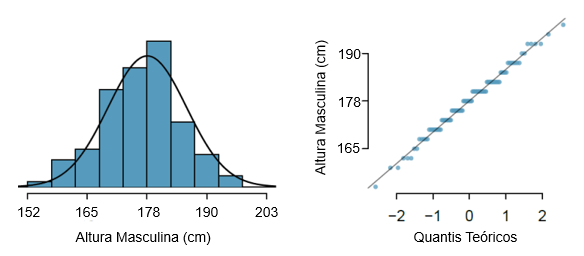
\includegraphics[width=0.9\textwidth]{3-2_evaluating_normal_approx/fcidMHeights.png}
\end{center}

\end{frame}

%%%%%%%%%%%%%%%%%%%%%%%%%%%%%%%%%%%%

\begin{frame}
\frametitle{Anatomia de um gráfico de probabilidade normal}

\begin{itemize}
\justifying
\item Os dados são plotados no eixo y de um gráfico de probabilidade normal e quantis teóricos (seguindo uma distribuição normal) no eixo x.
\justifying
\item Se houver um relacionamento linear no gráfico, os dados seguem uma distribuição quase normal.
\justifying
\item A construção de um gráfico de probabilidade normal requer o cálculo dos percentis e dos escores z correspondentes para cada observação, o que pode ser entediante. Portanto, geralmente dependemos de um software para fazer esses gráficos.

\end{itemize}

\end{frame}

%%%%%%%%%%%%%%%%%%%%%%%%%%%%%%%%%%%%

\begin{frame}
\frametitle{Exemplo}
\justifying
\dq{Abaixo está um histograma e um gráfico de probabilidade normal para as alturas da NBA da temporada 2008-2009. Esses dados parecem seguir uma distribuição normal?}

\begin{center}
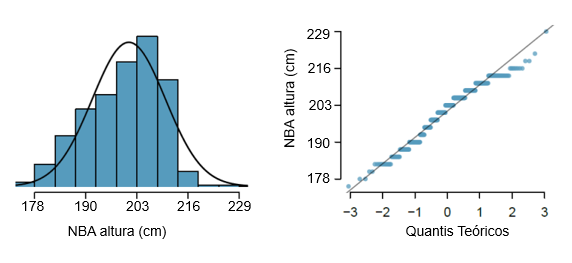
\includegraphics[width=0.8\textwidth]{3-2_evaluating_normal_approx/nbaNormal.png}
\end{center}

\pause
\justifying
\dq{Por que os pontos de probabilidade normal têm saltos?}

\end{frame}

%%%%%%%%%%%%%%%%%%%%%%%%%%%%%%%%%%%%

\begin{frame}
\frametitle{Gráfico de probabilidade normal e assimetria}

\twocol{0.2}{0.8}{
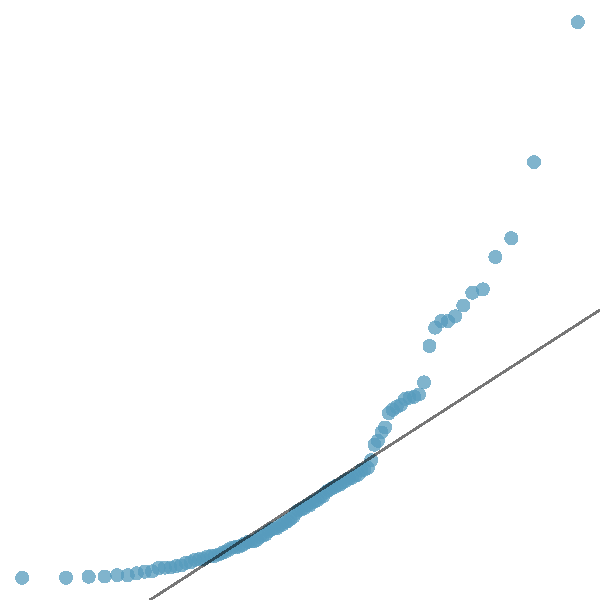
\includegraphics[width=0.8\textwidth]{3-2_evaluating_normal_approx/qq_rs.pdf}
}
{
\justifying
Inclinação à direita - Os pontos são curvados para cima e para a esquerda da linha.
}

\twocol{0.2}{0.8}{
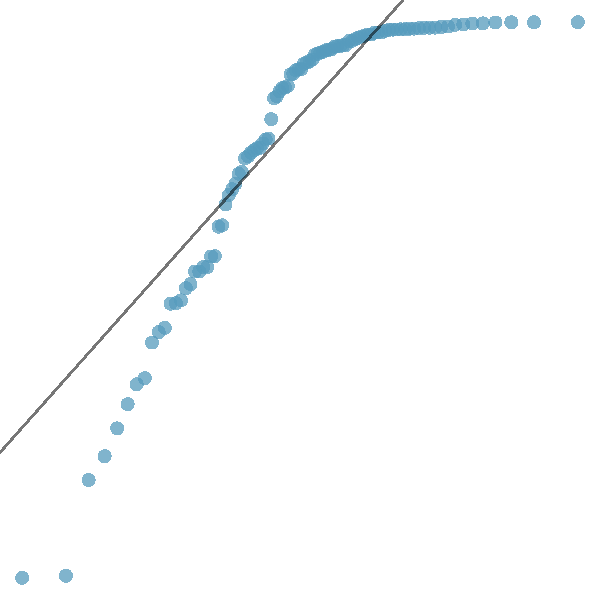
\includegraphics[width=0.8\textwidth]{3-2_evaluating_normal_approx/qq_ls.pdf}
}
{
\justifying
Inclinação da esquerda - Pontos curvados para baixo e para a direita da linha.
}

\twocol{0.2}{0.8}{
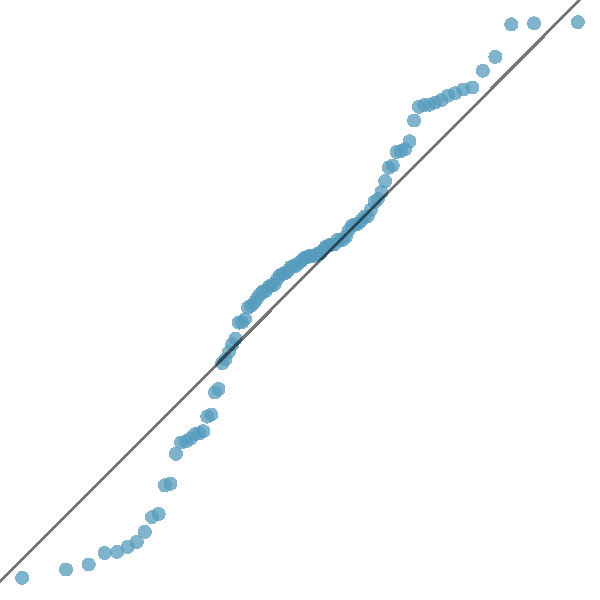
\includegraphics[width=0.8\textwidth]{3-2_evaluating_normal_approx/qq_st.pdf}
}
{
\justifying
Inclinação mais acentuada (mais estreitas que a distribuição normal) - Os pontos seguem uma curva em forma de S.
}

\twocol{0.2}{0.8}{
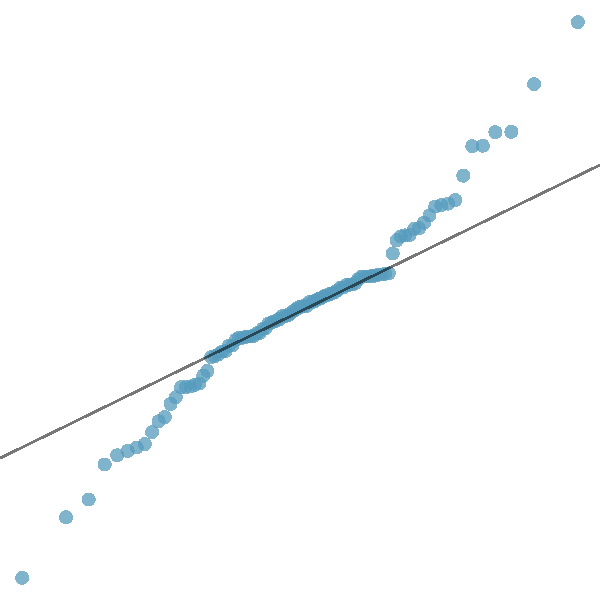
\includegraphics[width=0.8\textwidth]{3-2_evaluating_normal_approx/qq_lt.pdf}
}
{
\justifying
Inclinação menos acentuada (mais largas que a distribuição normal) - Os pontos começam abaixo da linha, passando a seguir a linha e terminam acima dela linha.
}

\end{frame}

%%%%%%%%%%%%%%%%%%%%%%%%%%%%%%%%%%%%

